\chapter{Serier}
En \underline{serie} defineras som en summa av oändligt många termer,
dvs. $s=\sum_{n=1}^\infty a_n=a_1+a_2+a_3+...$.
Rent formellt är $s=\lim_{N\to\infty}s_N$ där $s_N$ beteckna partialsumman $s_N=\sum_{n=1}^N a_n$ och man säger att $s$ är \underline{konvergent} om gränsvärdet $\lim_{N\to\infty}S_N$ existerar.
En \underline{geometrisk serie} definieras av egenskapen att kvoten mellan två på varandra närliggande termer är konstant,
dvs. $\frac{a_{n+1}}{a_n}=r$.
Det betyder att:
\begin{equation*}
    \left.
    \begin{matrix}
        a_1=a \\
        a_n=a\cdot r^{n-1}
    \end{matrix}
    \right\rbrace
    \Rightarrow\sum_{n=1}\infty a_n=a+a\cdot r+a\cdot r^2+...
\end{equation*}
För geometriska summor vet vi att:
\begin{equation*}
    s_N=a+a\cdot r+...+a\cdot r^{N-1}=\frac{a(1-r^N)}{1-r}
\end{equation*}
och om $-1<r<1$ (dvs $|r|<1$) så blir $\lim_{N\to\infty}s_N=\lim_{N\to\infty}\frac{a(1-r^N)}{1-r}=\frac{a}{1-r}$.
Villkoret att $|r|<1$ kallas för konvergenskriteriet (förutsatt att $a\neq 0$).
Rent allmänt hänger konvergens av serier ihop med de ingående termerna.

\paragraph{Sats} Om $\sum_{n=1}^\infty a_n$ konvergerar så måste $\lim_{n\to\infty}a_n=0$.
Annars om $\lim_{n\to\infty}a_n$ inte existerar eller inte är noll så kommer serien vara divergent.
\\
Räcker det med att $\lim_{n\to\infty}a_n=0$ för att avgöra konvergens av $s=\sum_{n=1}^\infty a_n$?
Nej, till exempel så divergerar den \underline{harmoniska serien} $\sum_{n=1}^\infty\frac{1}{n}$ mot $\infty$.
\paragraph*{Hur kan man testa konvergens?}
Kan tolka $\sum_{n=1}^\infty a_n$ som en "area" genom att tänka $\sum_{n=1}^\infty a_n=a_1\cdot 1+a_2\cdot 2+a_3\cdot 1+...$, dvs.
% infoga bild 1
%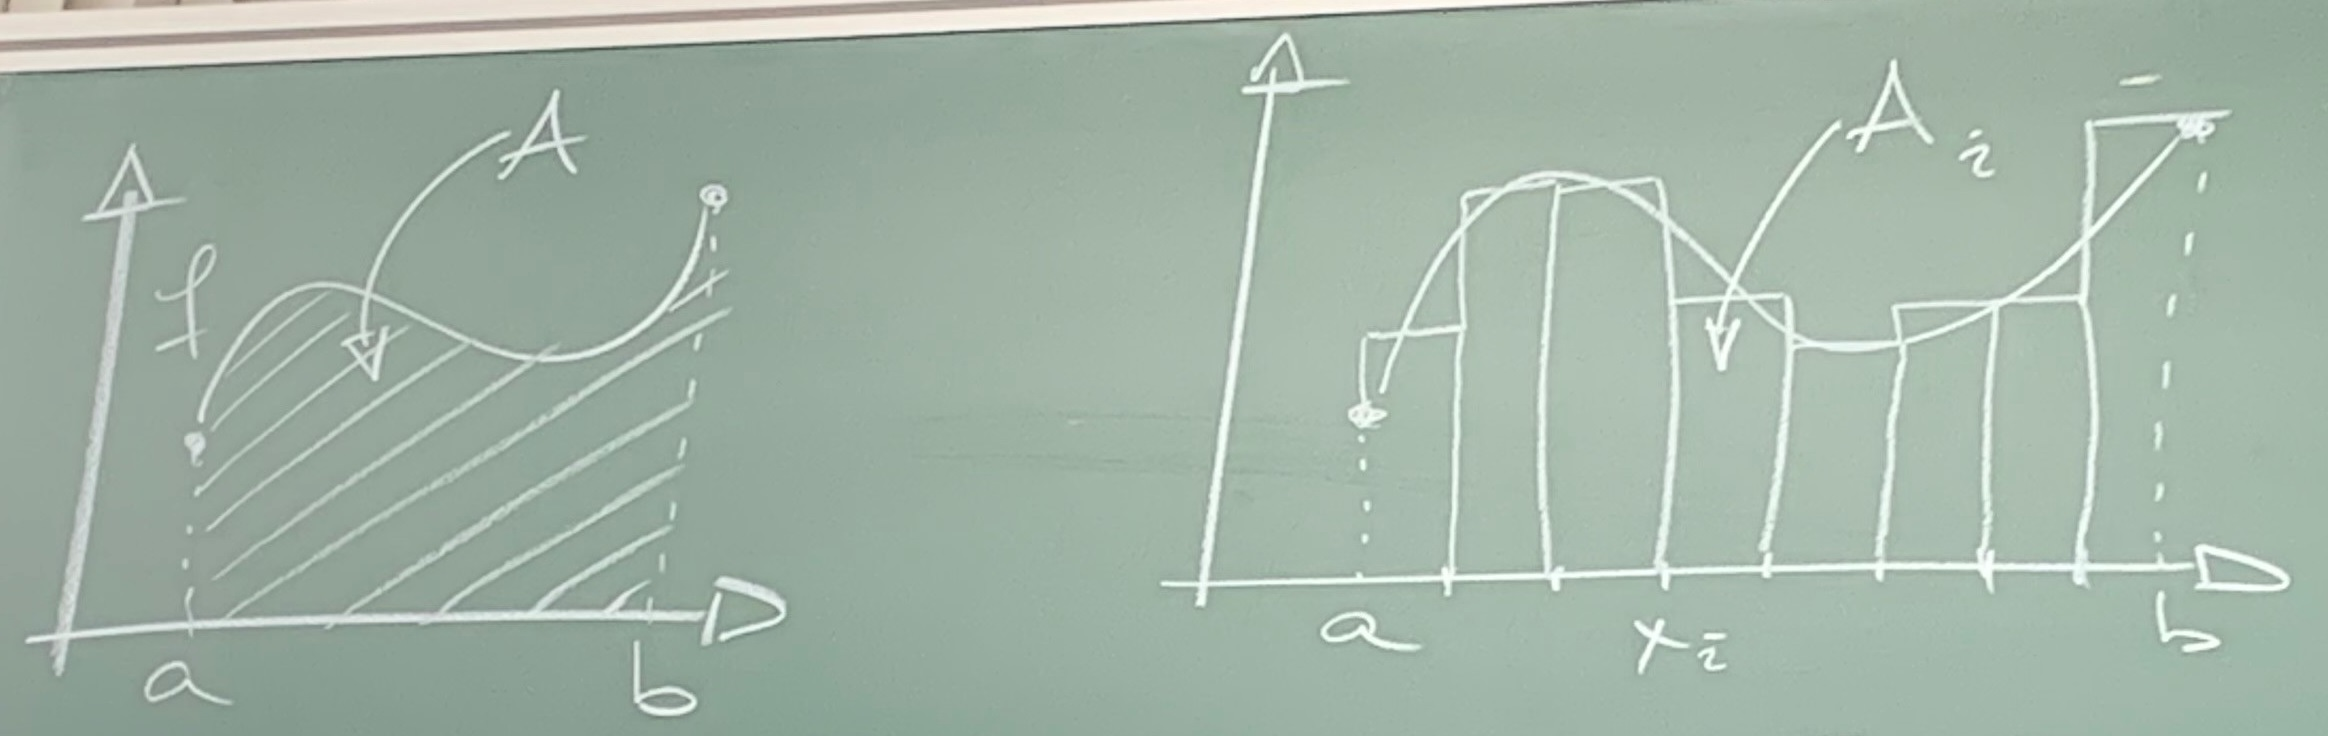
\includegraphics[]{lessons/lesson23/imgs/img01.jpg}
där stapel $i$ har bredd $1$ och höjd $a_i$.
Borde kunna uppskatta genom en integral om man kan hitta en funktion $f$ som löper genom staplarnas övre vänstra eller högra hörn?

\paragraph{Sats (integraltestet)}
Antag att $a_n=f(n)$ där funktionen $f$ är positiv, kontinuerlig och avtagande op ett intervall $[N,\infty)$ för något positivt heltal $N$.
Då kommer både $\sum_{n=1}^\infty a_n$ och $\int_n^\infty f(x)\, dx$ antingen att konvergera eller att divergera mot $\infty$. $\Box$
\\
Med hjälp av integraltestet kan man avgöra konvergens/divergens för p-serier genom jämförelse med p-integraler och får då
\begin{equation*}
    \sum_{n=1}^\infty n^{-p}=\sum_{n=1}^\infty\frac{1}{n^p}\,
    \left\lbrace
    \begin{matrix}
        \text{konv. om }p>1 \\
        \text{div. mot }\infty\text{ om }p\leq 1
    \end{matrix}
    \right.
\end{equation*}

\paragraph{Ex (9.3.5)} Avgör om serien $\sum_{n=1}^{infty}|\sin(\frac{1}{n^2})|$ är konvergent/divergent genom något lämpligt test.
\subparagraph*{Lösning}
Serien är uppenbart positiv och $|\sin(\frac{1}{n^2})|\to 0$ då $n\to\infty$.
Av taylors formel runt $a=0$ vet vi att $\sin(x)=x+\frac{(-\cos(s))}{6}\cdot x^3$ för något tal $s$ mellan $0$ och $x$.
Därför gäller att $\sin(\frac{1}{n^2})=\frac{1}{n^2}+\frac{(-\cos(s))}{6}\frac{1}{n^6}$ för något $s\in[0,\frac{1}{n^2}]$ och alltså har vi att
\begin{equation*}
    |\sin(\frac{1}{n^2})|=
    |\frac{1}{n^2}+\frac{(-\cos(s))}{6}\frac{1}{n^6}\leq
    \frac{1}{n^2}+|\frac{-\cos(s)}{6}|\frac{1}{n^6}\leq
    \{ | -\cos(s)|\leq 1\}\leq
    \frac{1}{n^2}+\frac{1}{6}\frac{1}{n^6}
\end{equation*}
Detta leder till att
\begin{equation*}
    \sum_{n=1}^\infty|\sin(\frac{1}{n^2})|\leq
    \sum_{n=1}^\infty(\frac{1}{n^2}+\frac{1}{6}\frac{1}{n^6})=
    \sum_{n=1}^\infty\frac{1}{n^2}+\frac{1}{6}\sum_{n=1}^\infty\frac{1}{n^6}
\end{equation*}
där båda serierna i högerledet är konvergenta enligt resultat för p-serier ($2>1$ och $6>1$) och alltså konvergerar vänsterledet! $\Box$
\\
En serie $\sum_{n=1}^\infty a_n$ sägs vara \underline{absolutkonvergent} om det gäller att $\sum_{n=1}^\infty |a_n|$ är konvergent.
Om däremot serien $\sum_{n=1}^\infty a_n$ är konvergent men \underline{inte} absolutkonvergent säger man att den är \underline{betingat konvergent}.
Till exempel är Serien
\begin{equation*}
    \sum_{n=1}^\infty\frac{(-1)^{n-1}}{n}=
    1-\frac{1}{2}+\frac{1}{3}-\frac{1}{4}+...
\end{equation*}
betingat konvergent eftersom den konvergerar men
\begin{equation*}
    \sum_{n=1}^\infty|\frac{(-1)^{n-1}}{n}=\sum_{n=1}^\infty\frac{1}{n}
\end{equation*}
är divergent mot $\infty$.

\section{Potensserier och Taylorserier}
Från den geometriska serien vet vi att
\begin{equation*}
    \sum_{n=1}^\infty r^{n-1}=
    1+r+r^2+...=
    \frac{1}{1-r}
\end{equation*}
förutsatt att $|r|<1$.
Kan därför skriva funktionen $f(x)=\frac{1}{1-x}$ där $|x|<1$, som en serie
\begin{equation*}
    f(x)=\frac{1}{1-x}=\sum_{n=1}^\infty x^{n-1}=1+x+x^2+x^3+...
\end{equation*}
Detta är ett exempel på en så kallad \underline{potensserie}.

\paragraph{Definition (Potensserie)}
En serie på formen
\begin{equation*}
    \sum_{n=0}^\infty a_n(x-c)^n=
    a_0+a_1(x-c)+a_2(x-c)^2+...
\end{equation*}
kallas för en potensserie i $(x-c)$ riunt punkten $x=c$.
\\
Vad gäller för potensegenskaper för potensserier?
\paragraph*{Sats}
För godtycklig potesnserie $\sum_{n=0}^\infty a_n(x-c)^n$ gäller alltid något utav följande:
\begin{enumerate}[label=(\roman*)]
    \item serien konvergerar bara $x=c$.
    \item serien konvergerar för alla $x\in\mathbb{R}$.
    \item det finns ett tal $R$ (kallas konvergensradien) så att serien konvergerar för alla $x$ så att $|x-c|<R$ och divergar för alla $x$ så att $|x-c| >R$.
          I ändpunkten där $|x-c|=R$ kan man ha antingen konvergens eller divergens.
\end{enumerate}
I $(i)-(iii)$ är konvergensen \underline{absolut} utom möjligtvis i ändpunkterna där \\
$|x-c|=R$.
För naturliga representationer av deriverbarar funktioner som potensserier genoma att uttrycka dom som "oändligt långa" Taylor-polynom runt given punkt $x=c$.
\begin{equation*}
    f(x)=\sum_{n=0}^\infty\frac{f^{(n)(c)}}{n!}(x-c)^n
\end{equation*}
Sådana serier, givet att de konvergerar för $x$ runt $c$,
kallas för Taylor-serier av $f$ runt $x=c$.
Några kända Taylor-serier runt $x=0$ (Maclaurin-serier) är:
\begin{enumerate}
    \item $e^x=\sum_{n=0}^\infty\frac{x^n}{n!}=1+\frac{x}{1!}+\frac{x}{2!}+\frac{x^3}{3!}+...$
    \item $\sin(x)=\sum_{n=0}^\infty\frac{(-1)^n}{(2n+1)!}x^{2n+1}=x-\frac{x^3}{3!}+\frac{x^5}{5!}-...$
    \item $\cos(x)=\sum_{n=0}^\infty\frac{(-1)^n}{(2n)!}x^{2n}=1-\frac{x^2}{2!}+\frac{x^4}{4!}-...$
\end{enumerate}
Om vi slarvar lite och betraktar $e^{2x}$ så får vi:
\begin{equation*}
    e^{ix}=
    \sum_{n=0}^\infty\frac{(ix)^n}{n!}=
    1+(ix)+\frac{(ix)^2}{2!}+\frac{(ix)^3}{3!}+...=
\end{equation*}
\begin{equation*}
    (1+\frac{(ix)^2}{2!}+\frac{(ix)^4}{4!}+\frac{(ix)^6}{6!}+...)+(ix+\frac{(ix^3)}{31}+\frac{(ix)^5}{5!}+...)=
\end{equation*}
\begin{equation*}
    (1-\frac{x^2}{2!}+\frac{x^4}{4!}-\frac{x^6}{6!}+...)+(ix+\frac{ix^3}{3!}+\frac{ix^5}{5!}-...)=
\end{equation*}
\begin{equation*}
    (1-\frac{x^2}{2!}+\frac{x^4}{4!}-\frac{x^6}{6!}+...)+i(x-\frac{x^3}{3!}+\frac{x^5}{5!}-\frac{x^7}{7!}+...)=
\end{equation*}
\begin{equation*}
    \cos(x)+i\sin(x)\text{, dvs. }
    e^{ix}=\cos(x)+i\sin(x)\text{ (Eulers formel!)}
\end{equation*}
Inte helt vattentätt eftersom detta resultat bygger på antagandet att Taylor-serier funkar på precis samma sätt för reella och komplexa tal.
För att helt förstå kopplingen måste man studera så kallade \underline{komplex matematisk analys}.
Vi nöjer oss här med Eulers formel och sambandet $e^{ix}=\cos(\pi)+i\cdot\sin(\pi)=-1$ alltså $e^{ix}=-1$.